\chapter{Original work}

In this chapter we explain the approach that was used to create a reinforcement learning agent that learns to play Briscola. The code implementation is available at \url{https://github.com/LetteraUnica/BriscolaBot}.

\begin{figure}[H]
    \centering
    \includesvg[width=0.9\textwidth]{images/general-architecture.svg}
    \caption{Starting from the Agent Pool, 4 opponents with frozen parameters are sampled. If the pool contains fewer than 4 agents, sampling is continued with replacement. The agent then plays 512 games against each opponent, resulting in a total of 2048 games (corresponding to 40960 tricks), which are played in parallel using a Vectorized Environment. During episode generation, the agent also collects experience and stores it in an Experience Buffer. Afterwards, the agent is trained on the collected experience using the PPO algorithm \cite{schulman2017proximal}. Finally, a copy of the updated agent is inserted into the Agent Pool with frozen weights. The process is repeated until the agent reaches the desired performance.}
    \label{fig:general-architecture}
\end{figure}
The general architecture \ref{fig:general-architecture} is composed of four main components, described in their respective sections in more detail:
\begin{itemize}
    \item \textbf{Vectorized Environment:} Implements the Briscola environment and allows for parallel execution of multiple games.
    \item \textbf{Agent Pool:} Stores a pool of agents with frozen weights. The agents are sampled during training to play against the agent being trained.
    \item \textbf{Experience Buffer:} Stores the experience collected by the agent during gameplay.
    \item \textbf{Optimization:} The agent is trained on the experience collected during gameplay using the PPO algorithm \cite{schulman2017proximal}.
\end{itemize}
After outlining the general architecture, we will explain the training process for the Briscola agent, along with the hyperparameters employed and performance evaluation. Ultimately, we will showcase the effectiveness of our approach by pitting the latest iteration of our agent, BriscolaBot-v3, against human players. To that end, interested readers can access the game at \url{https://replit.com/@LorenzoCavuoti/BriscolaBot}.

\section{Environment implementation}
To implement the environment we followed the guidelines of the PettingZoo library, which is a Python library for conducting research in multiagent reinforcement learning \cite{pettingzoo}. It is similar to OpenAI Gym, but it is designed for multiagent environments. We aimed to optimize the speed of the environment implementation to maximize the time spent in the training loop and minimize the time spent on executing game logic.

\subsection{Agent observation}
The agent has access to various information during gameplay, including the cards played so far, the cards in its hand, the Briscola card, the card on the table (if present), as well as its and the opponent's score. This information is represented in a vector with 162 components, as detailed in Table \ref{tab:state}.

\begin{table}[H]
    \centering
    \begin{tabular}{c c c c} 
     \hline
     Feature & n. components \\
     \hline
        Cards played & 40 \\
        Cards in hand & 40 \\
        Briscola card & 40 \\
        Table card & 40 \\
        \hline
        Agent points & 1 \\
        Opponent points & 1 \\
        \hline
        Total & 162 \\
        \hline
    \end{tabular}

    \caption{Features used as input to the agent in Briscola. The first set of features consists of one-hot encoded vectors, with each element indicating a card. For example, if a card has been played, the corresponding element is set to 1, while if it hasn't, it's set to 0. The same goes for the cards in hand, the Briscola card, and the card thrown by the opponent. The last two features show the agent's and opponent's scores, normalized by the highest possible score in Briscola to keep them within the range [0, 1].}
    \label{tab:state}
\end{table}

\subsection{Reward structure}
The reward structure is a weighted combination of two elements: win or loss and points earned in each turn:
\begin{equation}
    R = \alpha R_\textrm{win} + (1 - \alpha) R_\textrm{points}
    \label{eq:reward-structure}
\end{equation}
The reward structure consists of two terms: $R_\textrm{win}$ and $R_\textrm{points}$. $R_\textrm{win}$ is equal to 1 if the agent wins the game and 0 otherwise, and is only given at the end of the game. On the other hand, $R_\textrm{points}$ are the points the agent gains in each turn normalized by the highest possible score in Briscola and are given at every turn. The relative importance of these two terms is controlled by $\alpha$, which is a hyperparameter. Ideally, $\alpha=1$ should give the best results as it prioritizes winning. However, this can also lead to high variance in the reward structure and sparse rewards, with only 0 or 1 being given at the end of the game. In practice, we started training with $\alpha=0.1$ and the gradually increased it until we reached $\alpha=1$. This allows to learn fast a the beginning of training and then focus on winning the game.

\subsection{Action space}
We explored two different ways to represent the action space. The first representation consisted of three discrete actions, corresponding to each of the three cards the agent could play, making it an intuitive choice that mimics how humans play the game. In this representation all actions are valid except when near to the end of the game, where the player has fewer than 3 cards in hand. The second representation consisted of 40 discrete actions, each representing a card from the deck. This representation is less intuitive and most of the actions, around 93\%, are invalid. Despite these limitations, the second representation outperformed the first (as shown in Figure \ref{fig:action-space-comparison}). We believe this is because the agent doesn't have to consider the position of the cards in its hand and can instead focus solely on the cards it holds.
\begin{figure}[H]
    \centering
    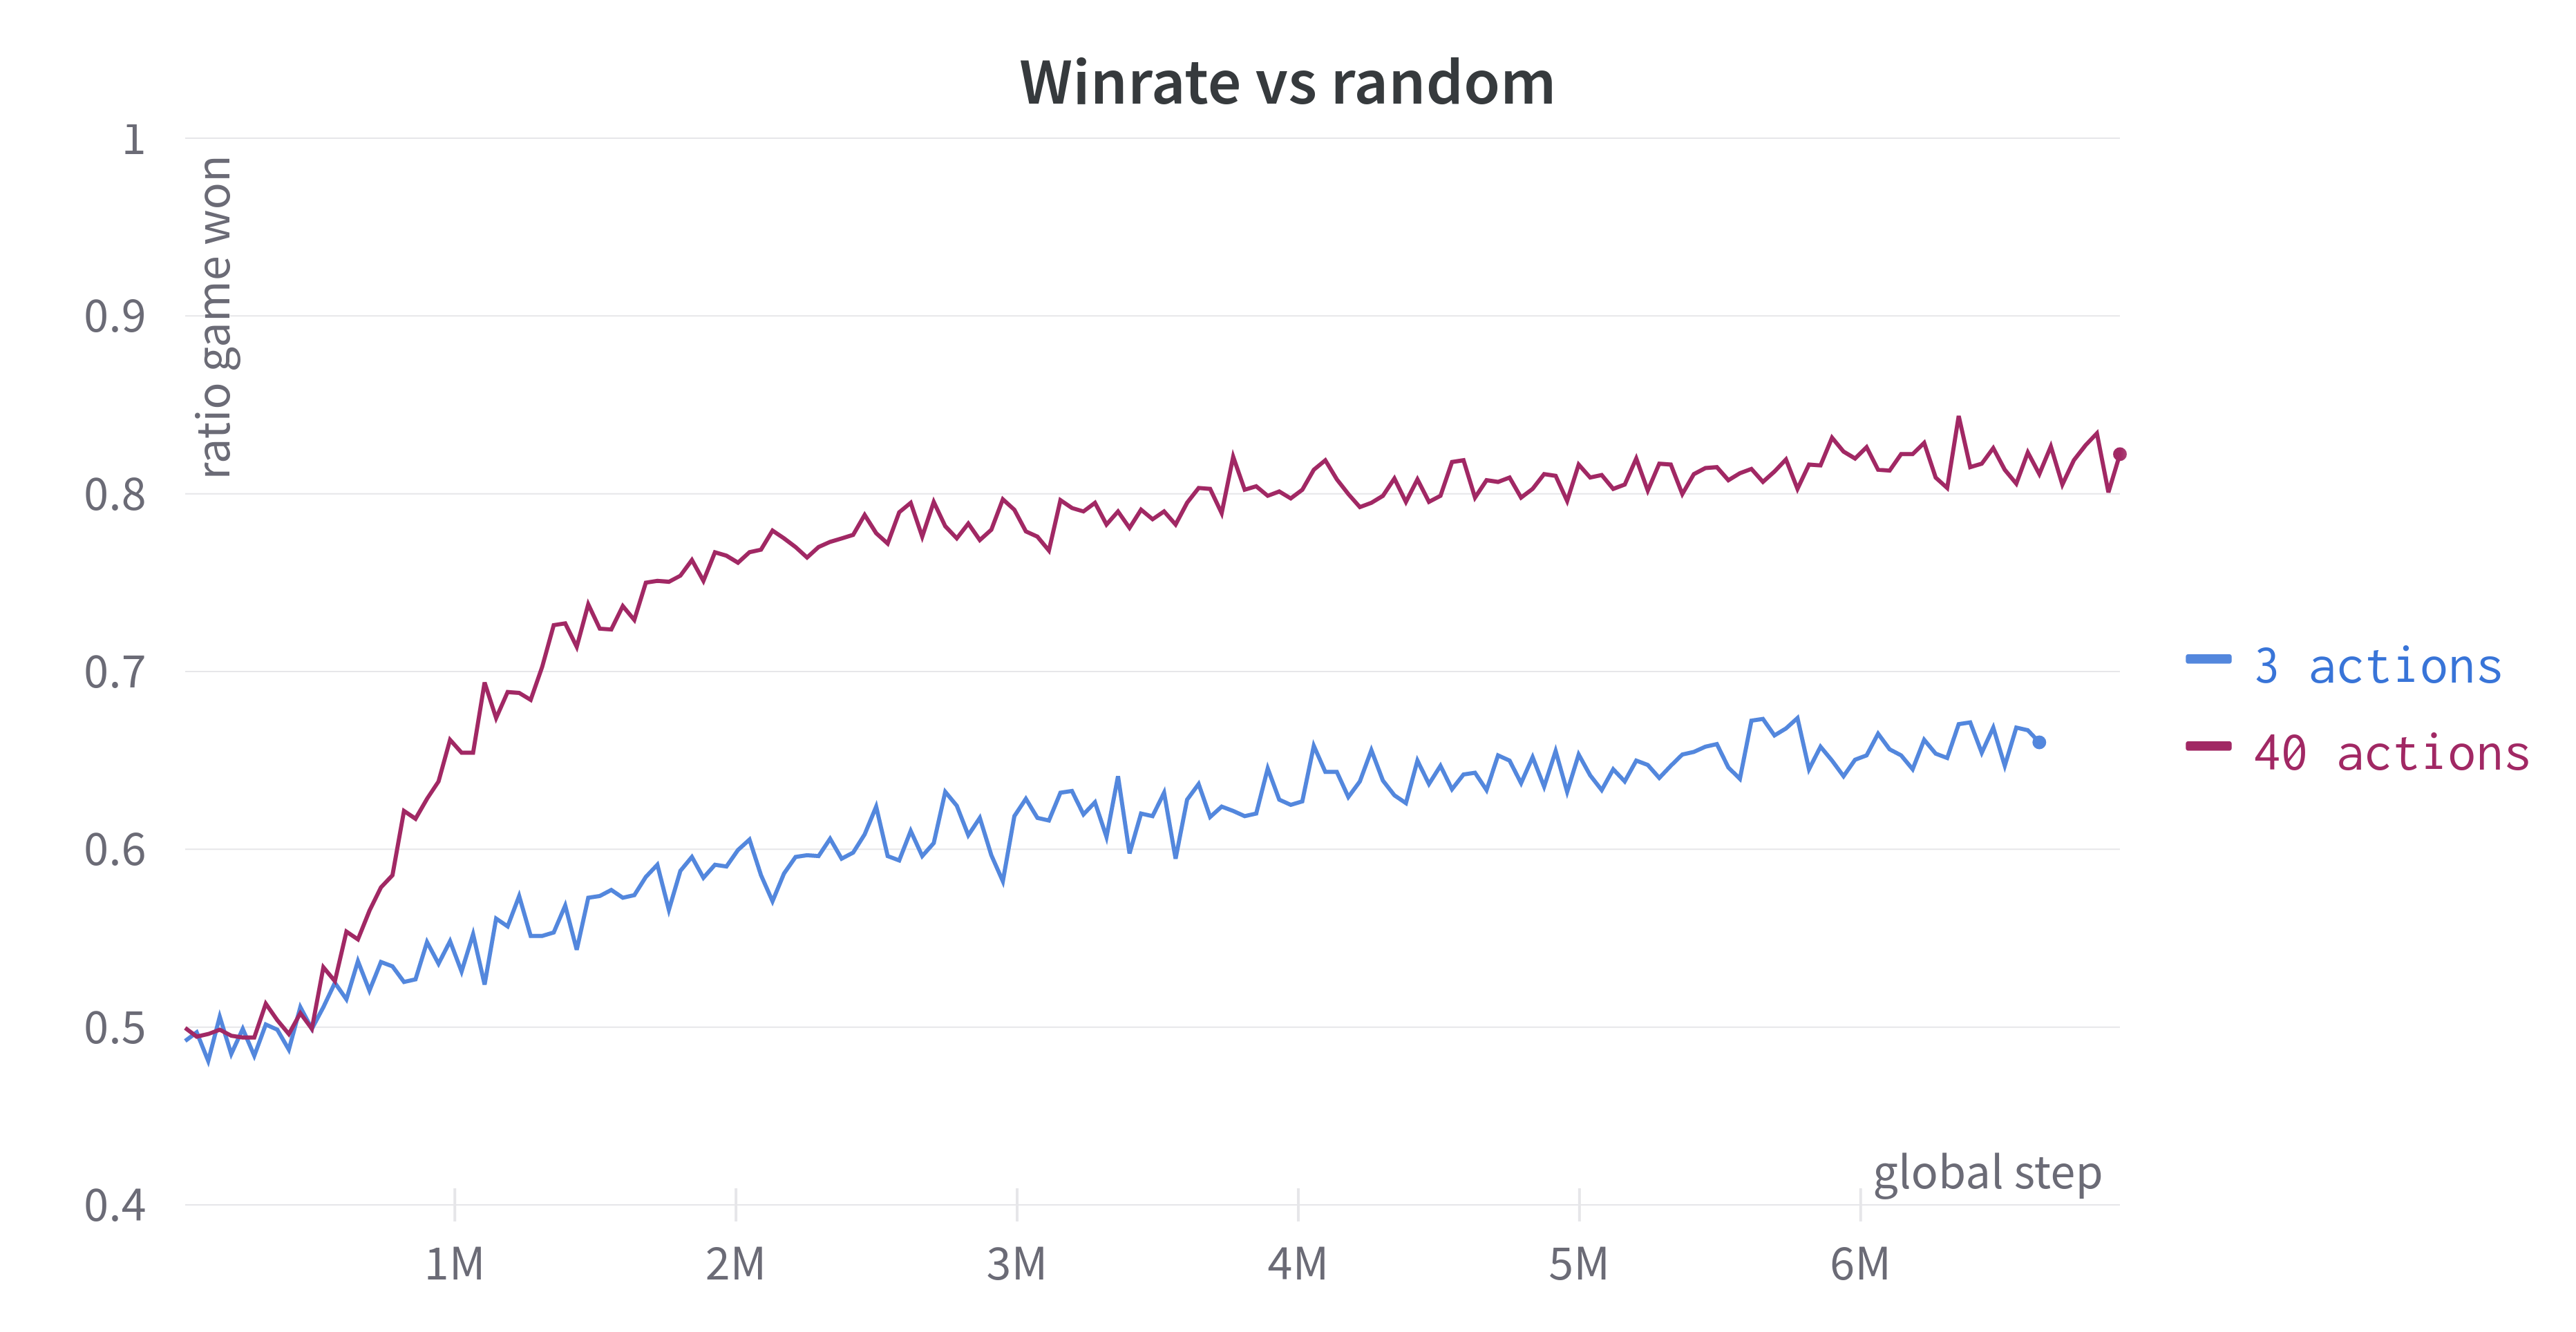
\includegraphics[width=\textwidth]{images/action-spaces-comparison.png}
    \caption{Performance of the two action space representations against a random player. The representation with 40 actions learns faster and reaches a win rate higher than 80\%, while the 3 action representation learns more slowly and reaches a win rate of 65\% by the end of training. In both representations we used invalid action masking as described in \cite{action-masking}.}
    \label{fig:action-space-comparison}
\end{figure}

\subsubsection{Invalid action masking}
Both in the first and second representation of the action space, the agent must not play a card that is not in its hand. This can be ensured through different methods, such as penalizing the agent for playing an invalid action or masking the invalid actions. We opted to implement the latter approach, as it has been shown empirically to be superior to penalizing invalid actions \cite{action-masking}.

The masking is done by setting the logits corresponding to the invalid actions to a small number, this way of performing the masking can be demonstrated to still produce a valid policy gradient as we are applying a differentiable state-dependent transformation to the policy \cite{action-masking}.

\begin{equation*}
    \pi'(\cdot|s) = \mathrm{softmax}(\mathrm{mask}(l_i))
\end{equation*}
\begin{equation*}
    \mathrm{mask}(l_{i}) = \begin{cases}
        l_i & \text{if $a_i$ is valid} \\
        M & \text{otherwise}
    \end{cases}
\end{equation*}
Where $l$ is the logits vector, $a$ is the action vector, $s$ is the state and $M$ is a small number, in our implementation we used $M=-10^6$.

\subsection{Vectorized environment}
In order to make the training process faster, we utilized a vectorized environment. This is a wrapper around the original environment that allows multiple instances of it to run simultaneously. In this setup, the agent receives all observations from all environments at once, which enables batching of policy evaluation and potentially performing it on a GPU, resulting in a significant speed-up of the training process.

\section{Agent}
When using policy-gradient methods the agent consists of two parts, the Actor and the Critic. The Actor, implemented as a multi-layer perceptron (MLP) with ReLU activations, defines the policy by mapping the agent's observation to a probability distribution over the action space (Figure \ref{fig:actor-critic-network}). On the other hand, the Critic uses the same MLP architecture as the Actor but outputs a single real value that represents the state's value (Figure \ref{fig:actor-critic-network}). We used two separate neural networks for the Actor and Critic as suggested in \cite{ppo-implementation-details}.

\begin{figure}[H]
    \centering
    \includesvg[width=0.6\textwidth]{images/actor-critic-net.svg}
    \caption{Diagram of the Actor-Critic Network Architecture. The Actor (left) transforms the agent's observation into a probability distribution over the 40 available actions, while the Critic (right) outputs a single real value, representing the state's value.}
    \label{fig:actor-critic-network}
\end{figure}

\section{Agent Pool}
The agent pool serves as a repository for past versions of the agent undergoing training, and keeps track of each version's win probability against the current agent. In detail, the pool holds a list of agents and their ratings $E_i$ against the agent being trained\footnote{The rating is very similar to the ELO system}. When opponents are selected for training, the pool samples them based on their ratings, with higher-rated agents having a higher probability of being chosen. This sampling is done using the following formula:

\begin{equation}
    P_i = \frac{e^{E_i}}{\sum_{j=1}^n e^{E_j}}
    \label{eq:agent-pool-sampling}
\end{equation}

The ratings of the opponents in the agent pool are updated after the agent has played games against them, with the following equation:

\begin{equation}
    E_i \rightarrow (1-\nu) E_i + \nu \, \textrm{logit}(\bar W_i)
    \label{eq:agent-pool-rating-update}
\end{equation}

Where $E_i$ represents the rating of opponent $i$, $\bar W_i$ is the average win rate of opponent $i$ against the agent being trained. The hyperparameter $\nu$ determines the influence of the old rating $E_i$ and the new rating $\textrm{logit}(\bar W_i)$ on the updated rating. If $\nu = 1$, the updated rating would be an unbiased estimator of the true rating. However, this would result in high variance. To reduce the variance, $\nu = 0.1$ is used, which biases the estimator towards $E_i$, reducing its variance.\\\\
The agent pool is a crucial component as it prevents the agent from forgetting how to overcome previous versions of itself. With the agent pool, the agent is exposed to a diverse range of opponents, including those it has previously defeated, and must be able to overcome them once again, thus ensuring its overall improvement.

\section{Optimization}
The optimization process is done using a variant of the Proximal Policy Optimization (PPO) algorithm, which includes several modifications that have been shown to improve the performance of the algorithm \cite{ppo-implementation-details}. Some of them are:
\begin{itemize}
    \item The learning rate decreases gradually during training, a common practice in deep learning that has been shown to also enhance PPO's performance.
    \item Generalized Advantage Estimation (GAE): The advantage function is calculated using GAE \cite{schulman2015high}, reducing variance in the advantage function and shortening training time.
    \item Normalization of Advantages: After GAE is used to calculate the advantages, they are normalized at the mini-batch level to have mean zero and unit variance. This operation doesn't change the policy gradient, but it helps the optimization process as the data is centered around zero.
    \item Loss entropy bonus: The loss function is enhanced with an entropy bonus, encouraging exploration and preventing the policy from becoming too deterministic too early in training.
\end{itemize}

The optimization of the agent is performed using the Adam optimizer \cite{kingma2014adam}, with a starting learning rate of $3 \cdot 10^{-3}$, which gradually decreases to $1 \cdot 10^{-4}$ during the training process. To accelerate training, a large batch size of 1024 to 2048 is employed, as it has been observed to increase efficiency, and it aligns with the typical use of large batch sizes in reinforcement learning \cite{mccandlish2018empirical}. The agent's performance is optimized by minimizing the following loss function.

\begin{equation}
    L = L_{\textrm{policy}} + \beta_\textrm{v} L_\textrm{value} - \beta_\textrm{e} L_\textrm{entropy}
    \label{eq:ppo-loss}
\end{equation}
In equation \eqref{eq:ppo-loss}, $L_{\textrm{policy}}$ represents the PPO policy loss as in equation \eqref{eq:ppo-update-clip}, $L_\textrm{value}$ is the mean squared error between the predicted value and the actual episode return, and $L_\textrm{entropy}$ is the entropy of the policy. The hyperparameters $\beta_\textrm{v}$ and $\beta_\textrm{e}$ control the relative importance of these terms and are commonly set around $0.5$ and $0.01$ respectively.

\section{Training Procedure}
We trained three agents with increasing level of performance using an incremental approach, similar to the one used when developing chess engines \cite{stockfish,lc0}. More in detail, when developing the next version of Stockfish, the developers measure its performance against the previous version, if the new version wins more games than the previous version, it is considered an improvement. This is a simple yet powerful approach as it allows to test the agent improvement without having to define an ELO rating, which can be hard to do, as it depends on the distribution of the opponents.

\subsection{BriscolaBot-v1}
The first version of the agent didn't use self-play with the agent pool, instead was only trained against a random opponent for 10 million steps. Before starting the final training run, however, we performed an extensive hyperparameter search using the Weights \& Biases bayesian search method \cite{wandb}. The algorithm was tasked to maximize the win probability against a random opponent in 1 million training steps. The method successfully discovered hyperparameters that reduced the time taken to reach an 80\% win rate against a random agent by half, as depicted in Figure \ref{fig:hyperparam-best-default}. The optimized hyperparameters are displayed in Table \ref{tab:hyperparam-best}.

\begin{figure}[H]
    \centering
    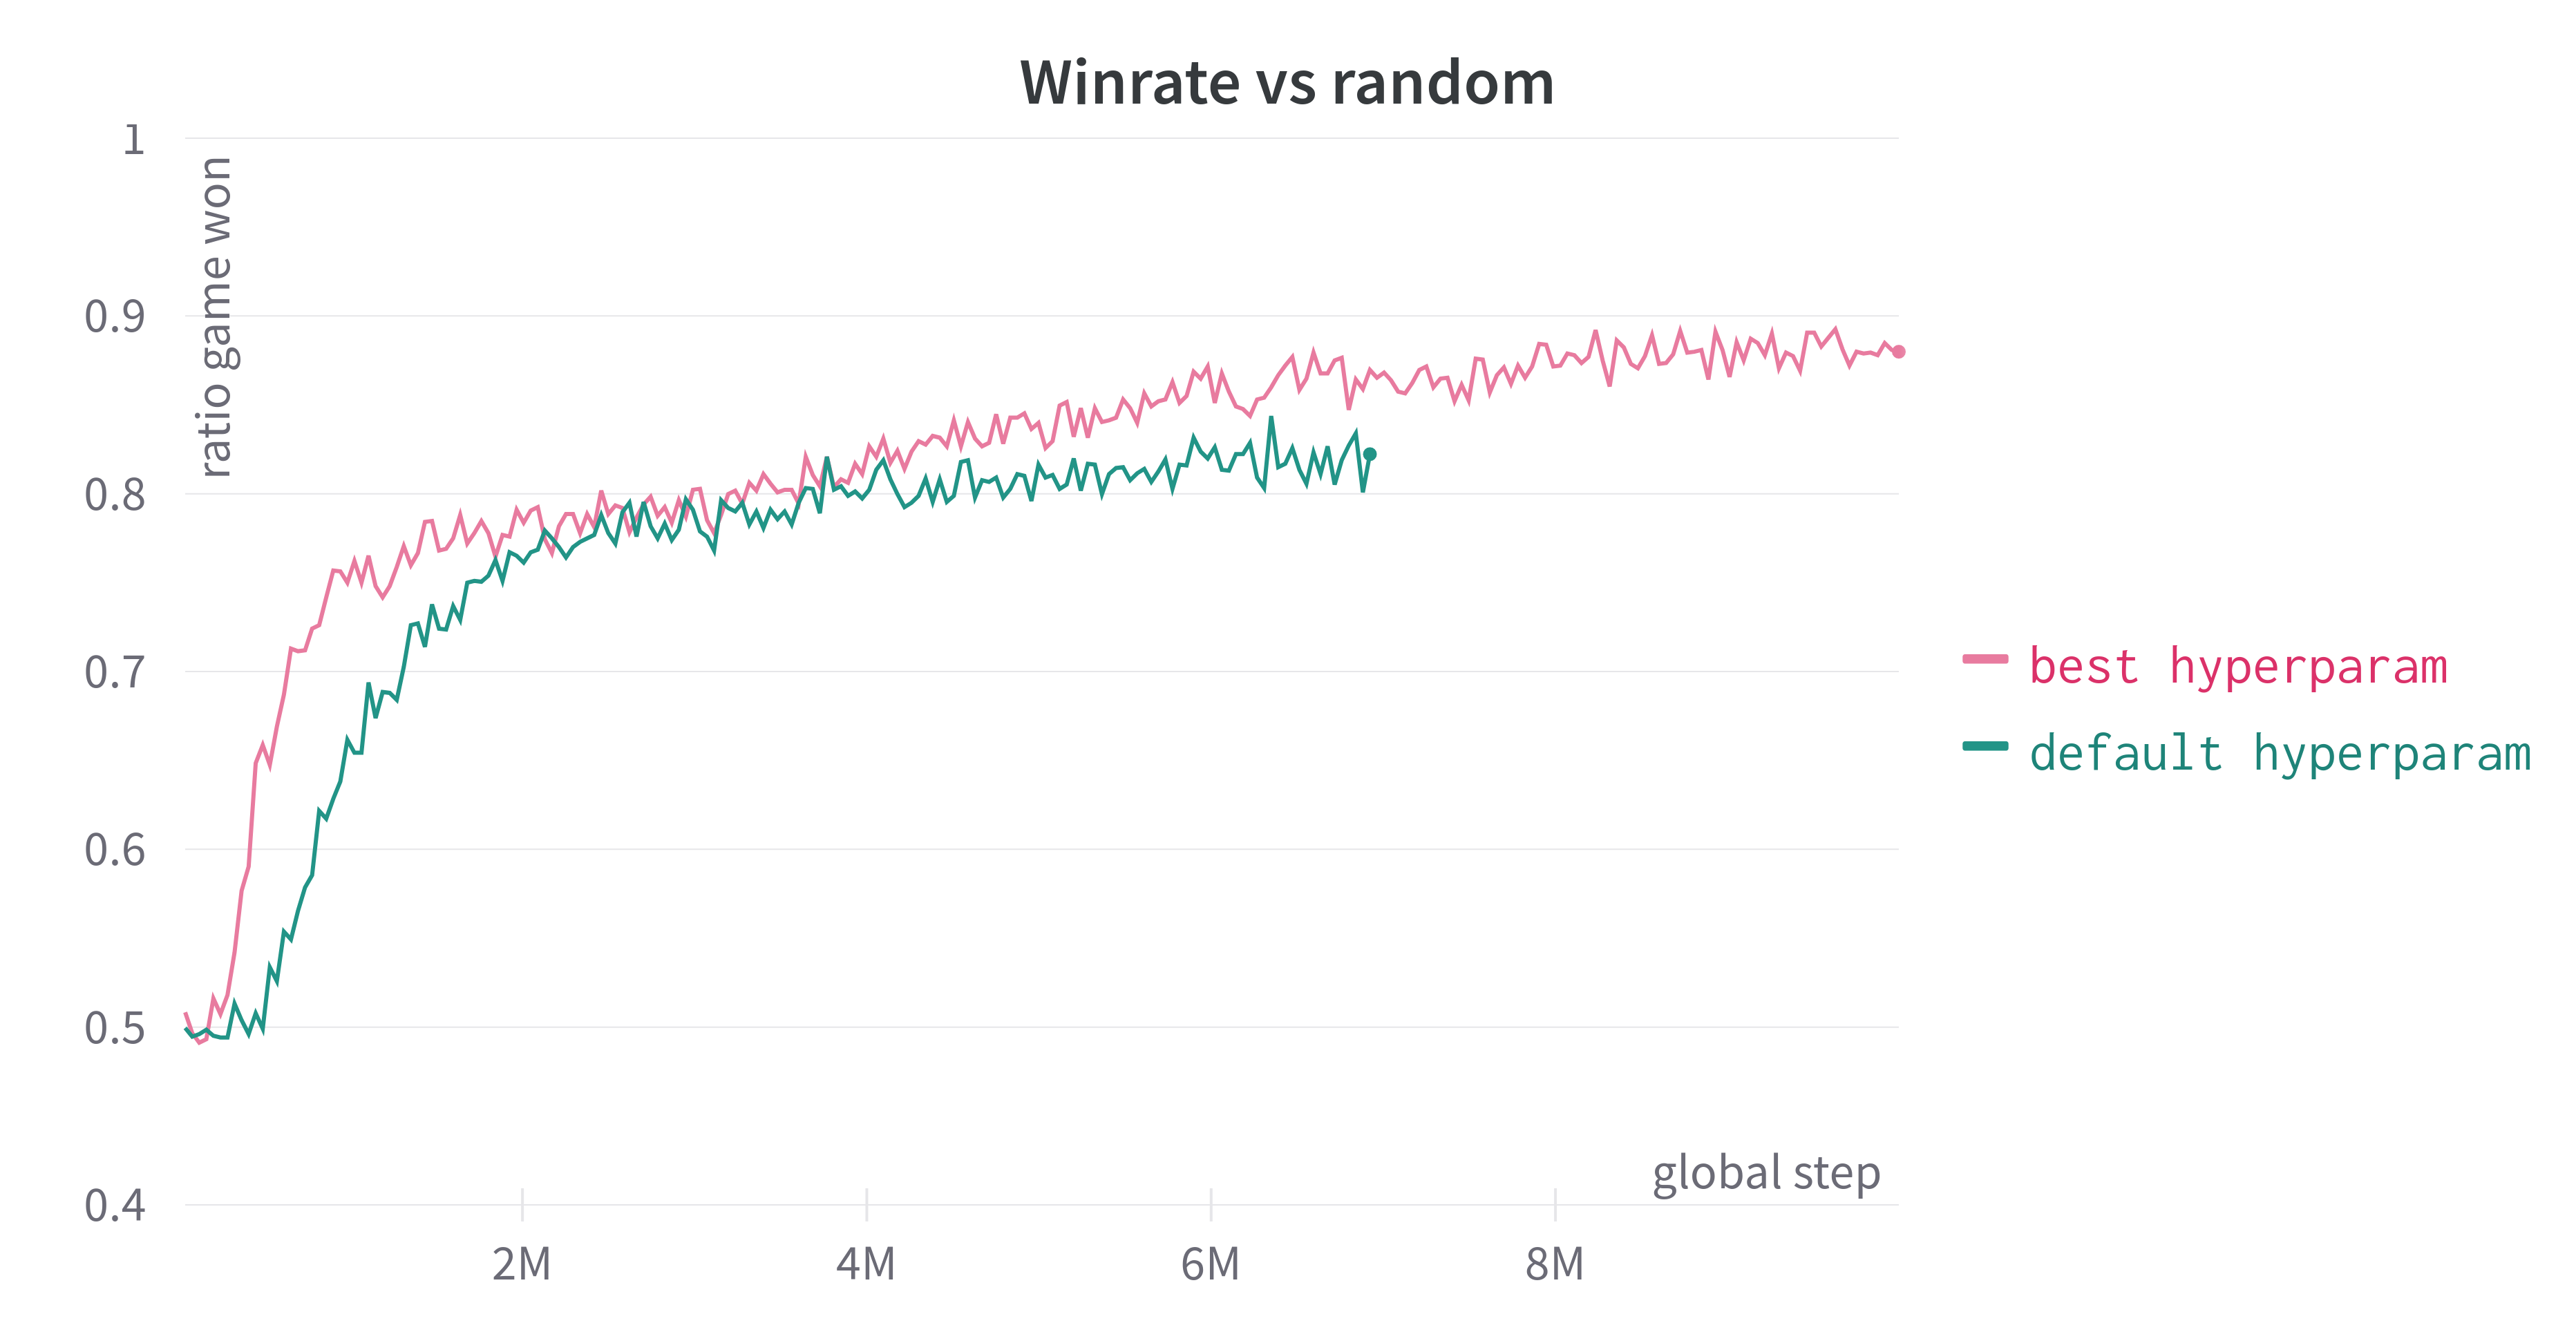
\includegraphics[width=\textwidth]{images/hyperparam-best-default.png}
    \caption{Comparison of the default hyperparameters and the best hyperparameters found using Weights \& Biases bayesian search method.}
    \label{fig:hyperparam-best-default}
\end{figure}

\begin{table}[H]
    \centering
    \begin{tabular}{ccc}
        \hline
        Hyperparameter & Default value & Best value \\
        \hline
        Learning rate & 0.001 & 0.003 \\
        Clip coefficient \eqref{eq:ppo-update-clip} & 0.2 & 0.3\\
        Entropy bonus \eqref{eq:ppo-loss} & 0.001 & 0.01 \\
        GAE $\lambda$ \eqref{eq:gae-advantage} & 0.95 & 0.9 \\
        Discount factor $\gamma$ \eqref{return-recursive} & 1 & 1 \\
        Ratio win reward $\nu$ \eqref{eq:reward-structure} & 0 & 0.1 \\
        Update epochs & 4 & 2 \\
    \end{tabular}
    \caption{Best hyperparameters found using Weights \& Biases bayesian search method. The default parameters were taken from the CleanRL implementation of PPO \cite{huang2022cleanrl} which provide a good starting point for reinforcement learning tasks. Update epochs is the number of passes over the collected episode data the optimization process performs.}
    \label{tab:hyperparam-best}
\end{table}

The final training run, which produced BriscolaBot-v1, was performed using the optimized hyperparameters. The agent was able to achieve a win rate of 80\% against a random agent in 1 million steps and almost 90\% in 10 million steps, as shown in figure \ref{fig:hyperparam-best-default}.

\subsection{BriscolaBot-v2}
In the second version of the agent, we added self-play with the agent pool, because the agent manages beat to a random opponent very quickly. Furthermore, we increased the neural network size to 256, changed the activation function from ReLU to Mish \cite{misra2019mish} and added learning-rate decay. The effect of some of these changes can be seen in figure \ref{fig:mish-activation}. After these changes, the agent was able to beat BriscolaBot-v1 60\% of the time when trained for 10 million steps, which is a good result considering the randomness of the game of Briscola.

\begin{figure}[H]
    \centering
    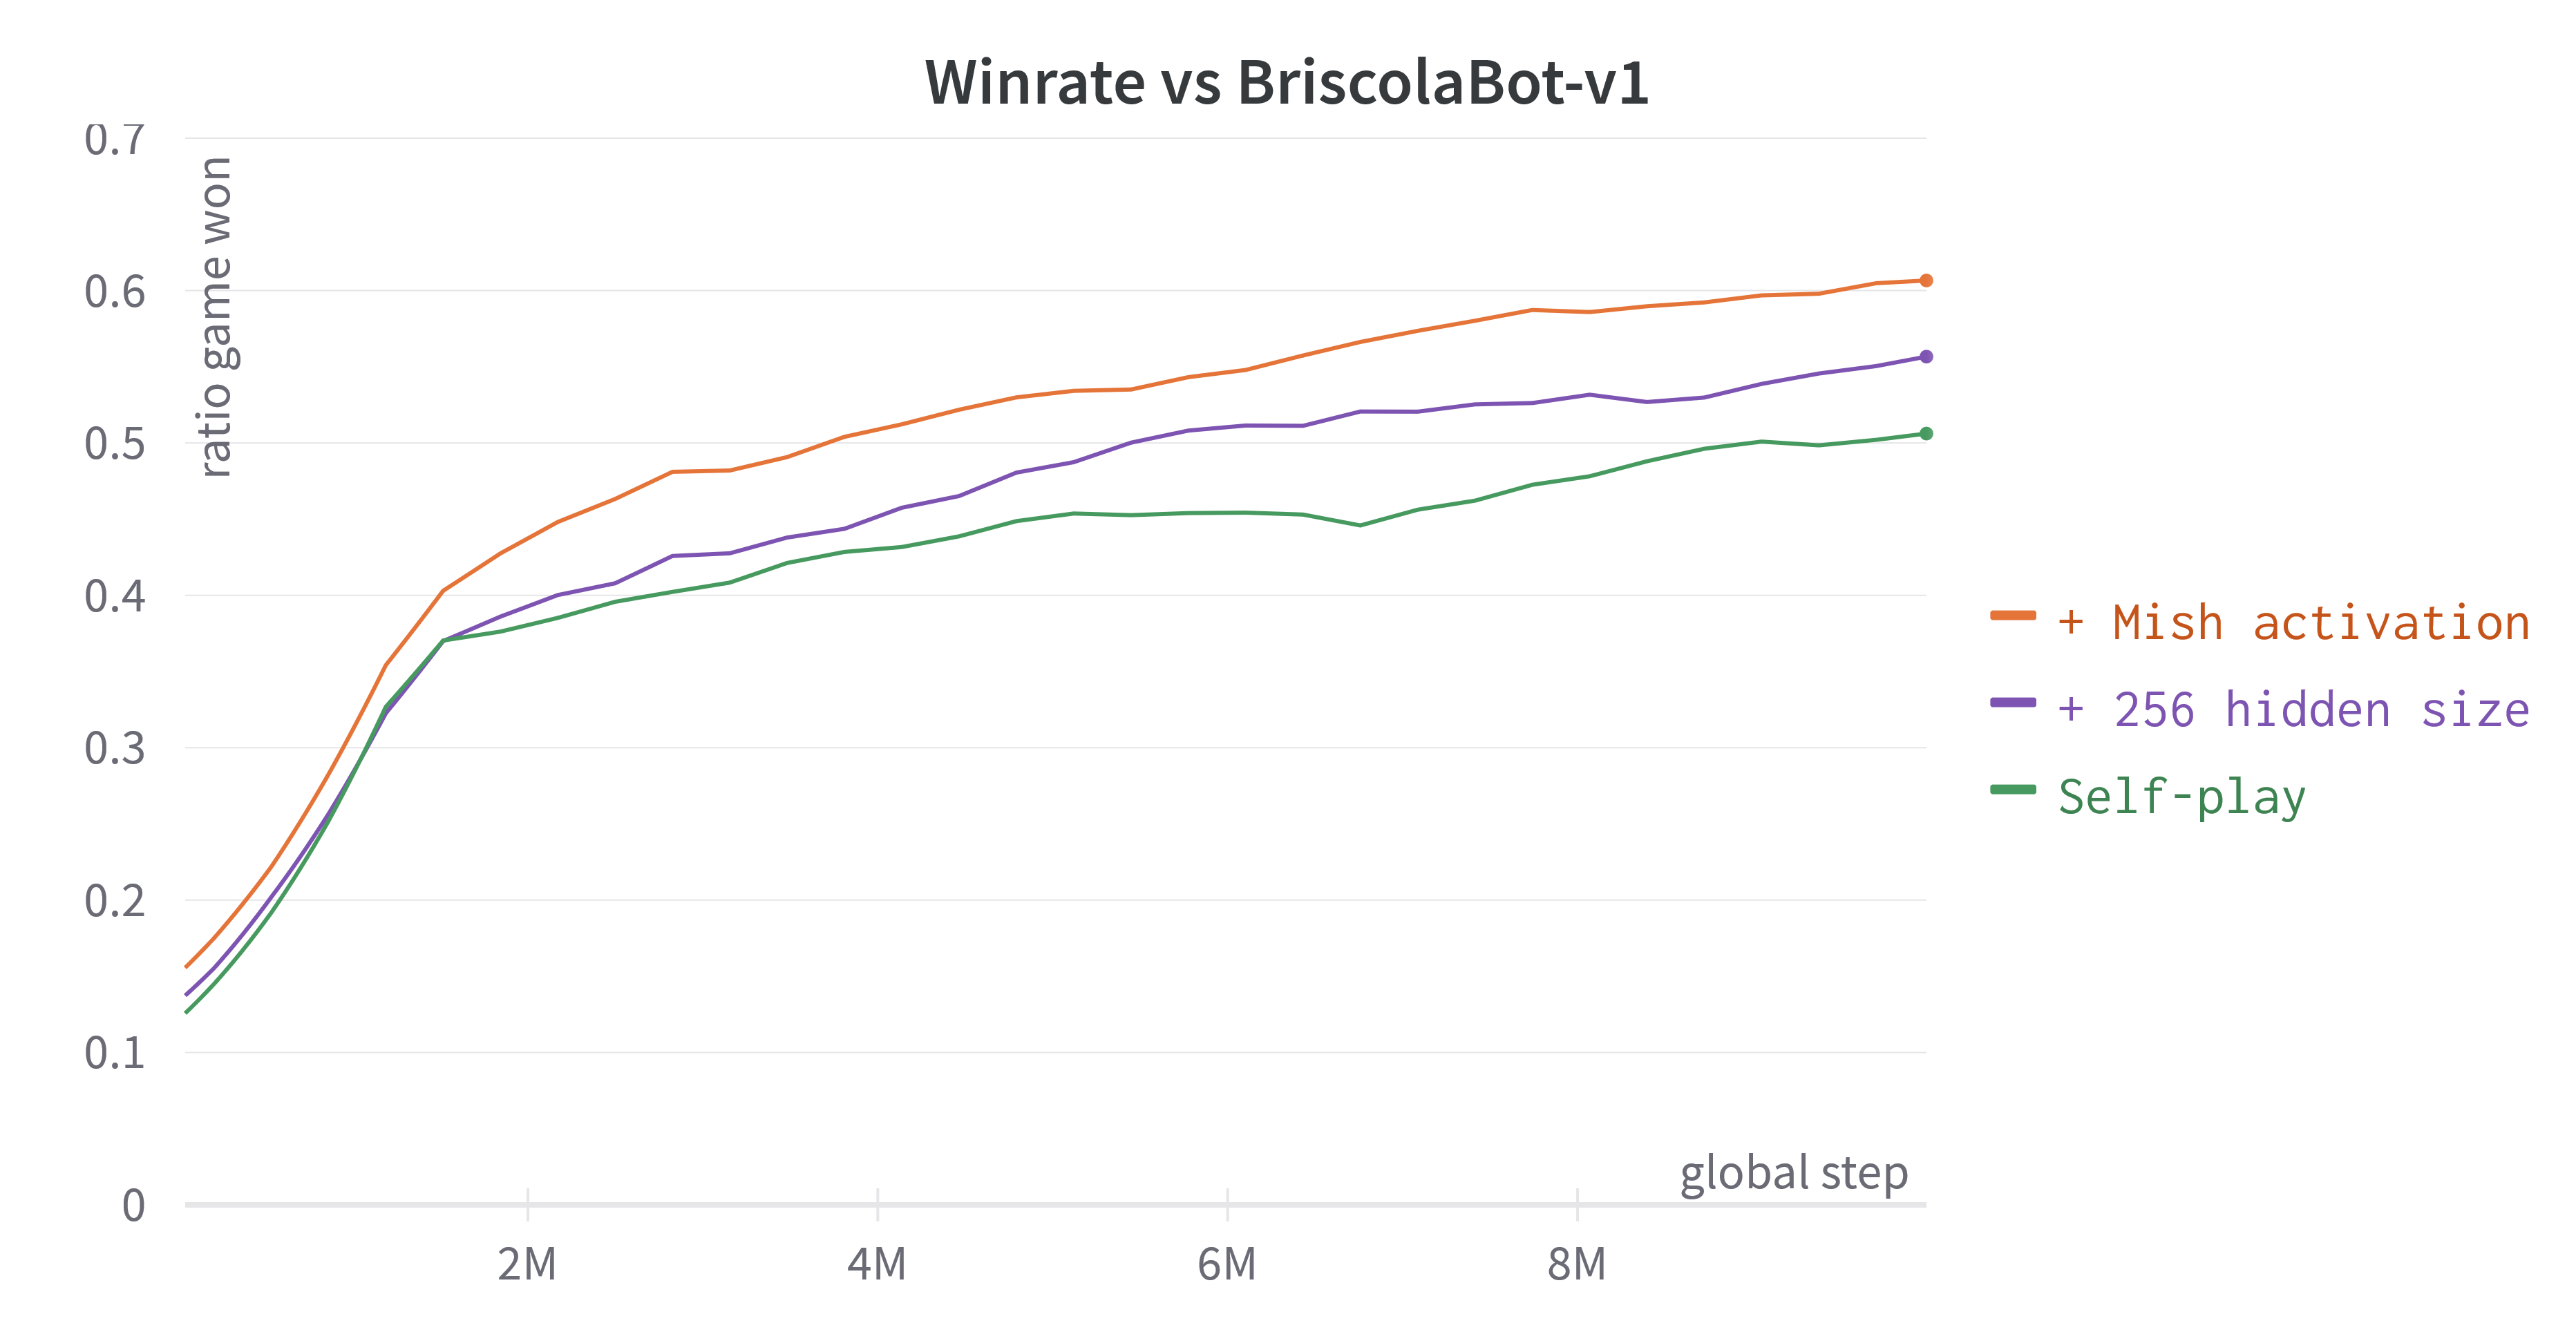
\includegraphics[width=\textwidth]{images/mish-activation.png}
    \caption{Win rate against BriscolaBot-v1 when adding self-play (green line), then increasing the neural network size from 128 to 256 (purple line) and on top of that changing the activation function from ReLU to Mish (orange line).}
    \label{fig:mish-activation}
\end{figure}

To produce the final version of the BriscolaBot-v2 agent we continued training until 20 million steps. BriscolaBot-v2 was able to achieve a win rate of 90\% against a random agent and 64\% against BriscolaBot-v1.

\subsection{BriscolaBot-v3}
A problem with BriscolaBot-v2 is that it throws the ace and the 3 of briscola very often, instead of waiting for the right opportunity. This is a problem, because the ace and the 3 of briscola are the most powerful cards in the game, and wasting them can lead to a loss.\\\\
We think that this problem is caused by giving too much importance to the number of points scored in the loss function \eqref{eq:reward-structure}, which might cause the agent to collect points as soon as possible. In this version, we tried to address this problem by gradually increasing the $\nu$ parameter in equation \eqref{eq:reward-structure} from 0.1 up to 1 during training. Another change that we applied was to decay the entropy $\beta_\textrm{e}$ parameter in equation \eqref{eq:ppo-loss} from 0.01 down to approximately zero, as this is an exploration parameter and should decrease when reaching optimal play \cite{open-ai-five}. The effect of these changes can be seen in figure \ref{fig:briscolabot-v3}.

\begin{figure}[H]
    \centering
    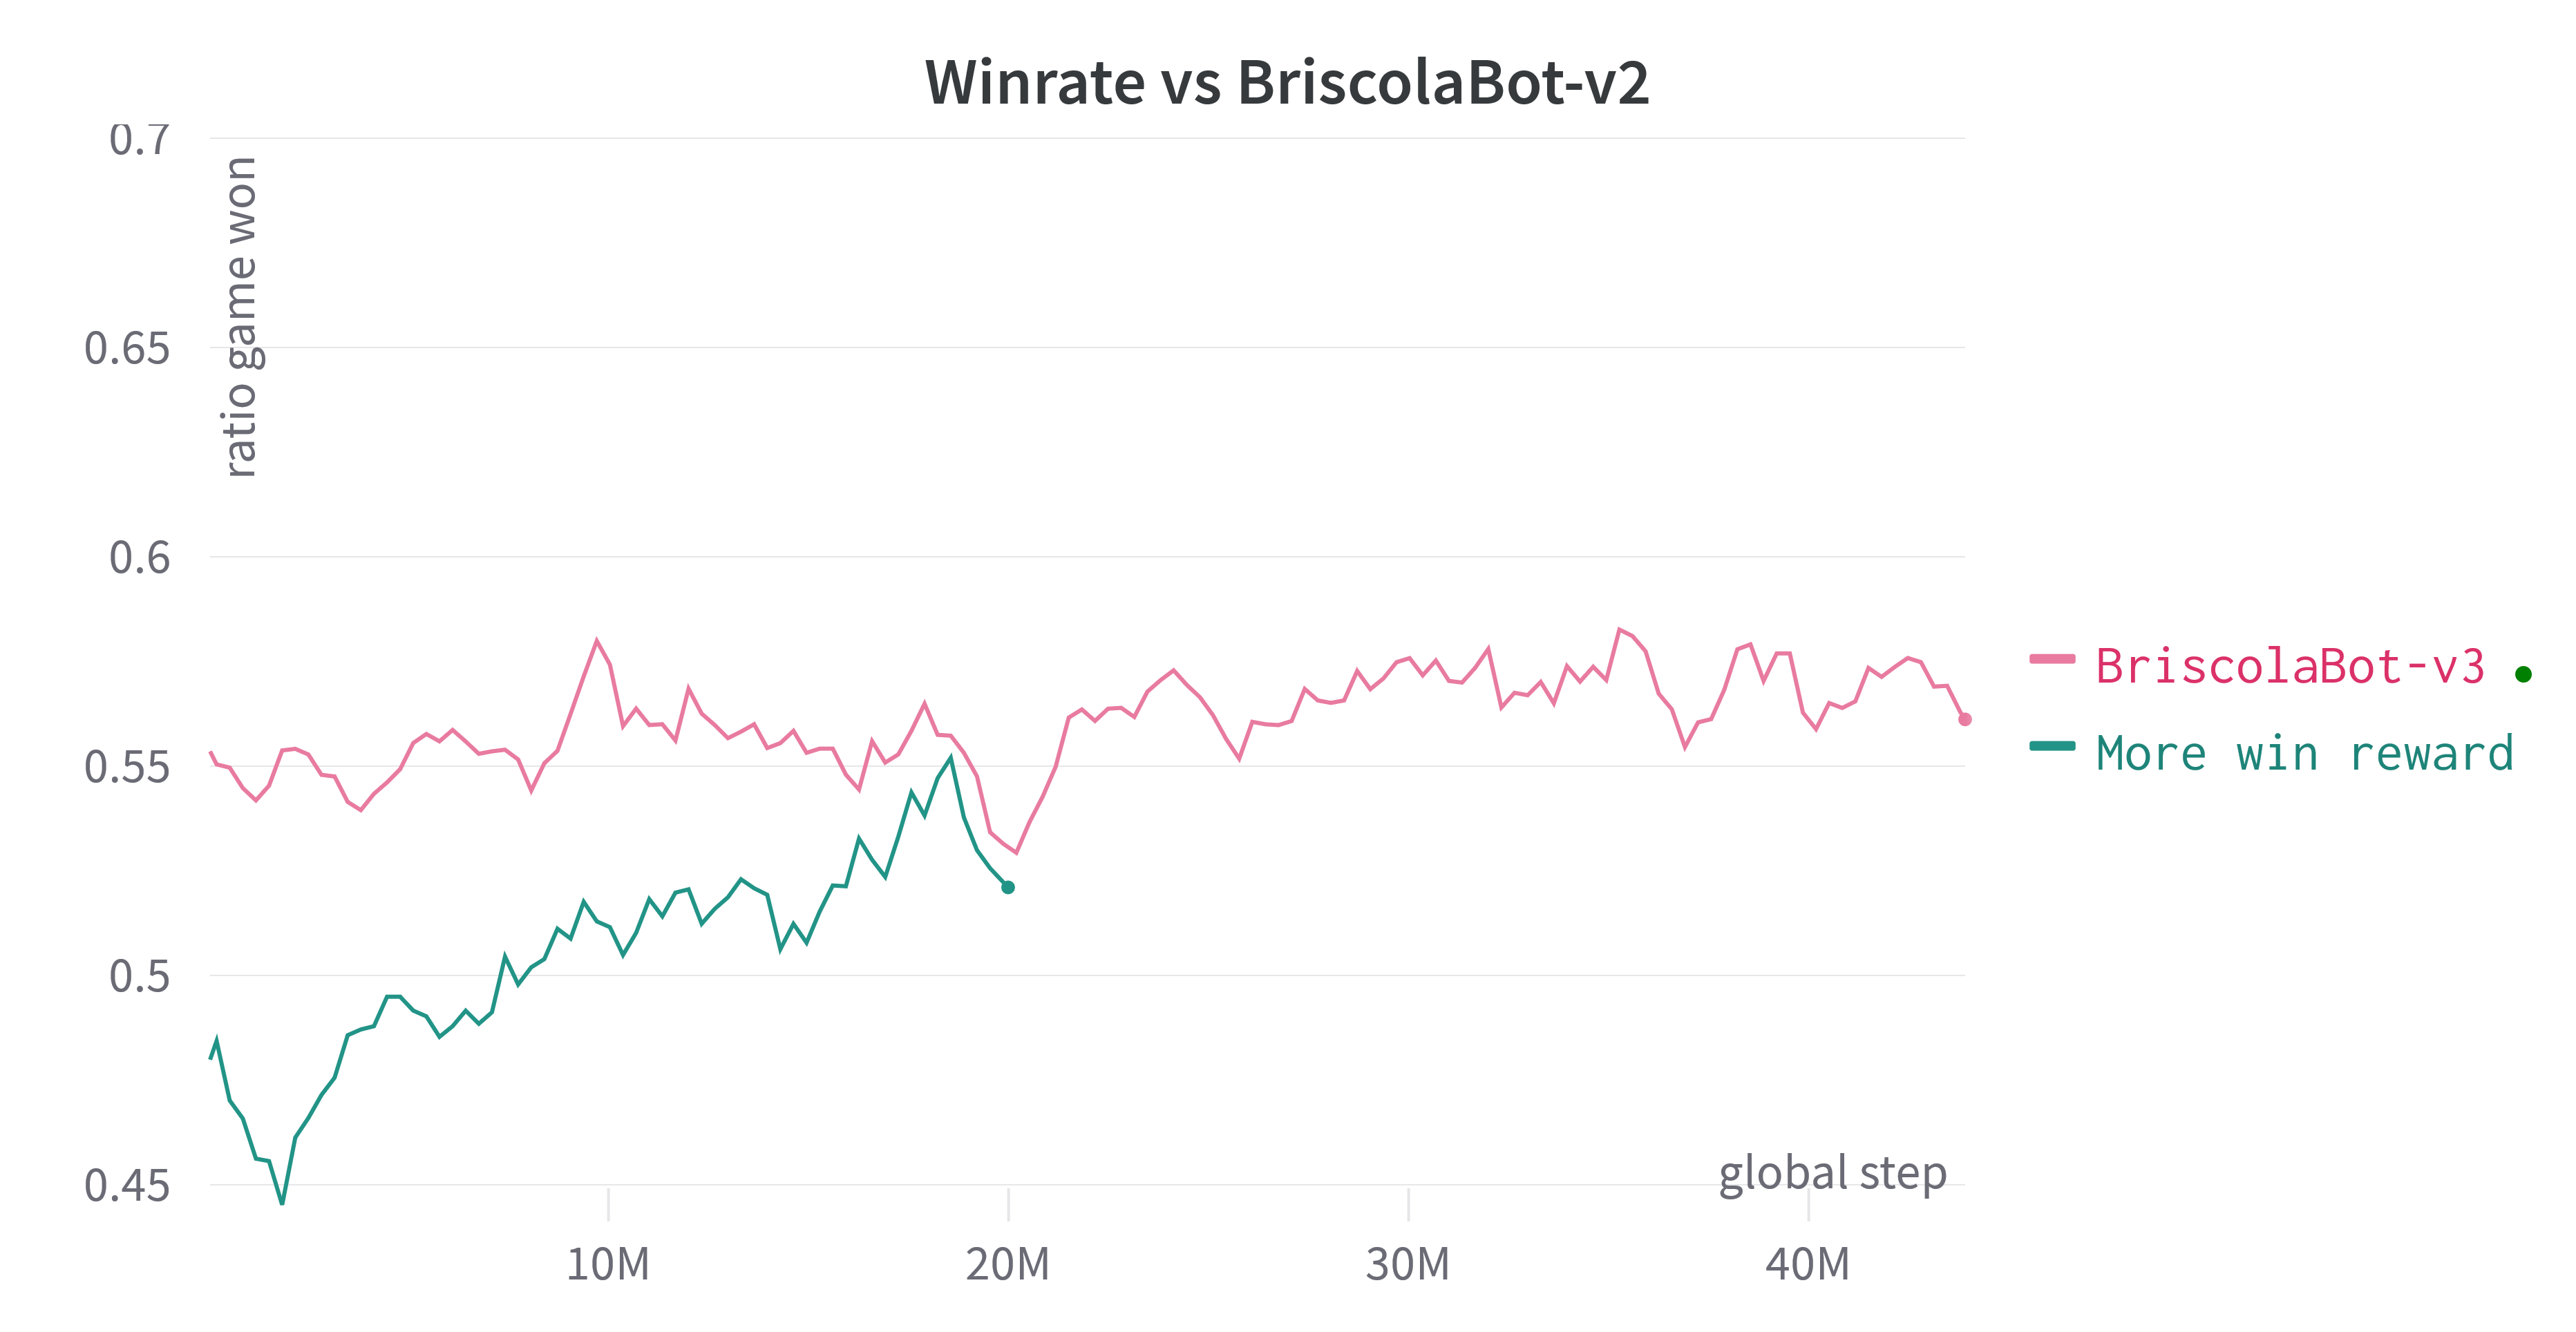
\includegraphics[width=\textwidth]{images/briscolabot-v3.png}
    \caption{Winrate against BriscolaBot-v2 when gradually increasing the $\nu$ parameter in equation \eqref{eq:reward-structure} and decreasing the entropy during training, we can see that these two changes improved the performance of the agent. Since these two runs started from the weights of BriscolaBot-v2, the ratio of games won starts near 0.5.}
    \label{fig:briscolabot-v3}
\end{figure}

The final agent was trained starting from the BriscolaBot-v2 weights, with the modifications listed above for 50 million steps, corresponding to approximately 4 hours of training on an Intel i5-4690K CPU. The agent was able to achieve a win rate of 57\% against BriscolaBot-v2 and 93\% against a random agent, surpassing previous approaches to the problem \cite{alsora-deep-briscola-dqn}. The final list of hyperparameters used for the final agent is shown in Table \ref{tab:hyperparam-final}.

\begin{table}[H]
    \centering
    \begin{tabular}{cccc}
        \hline
        Hyperparameter & Value & Hyperparameter & Value \\
        \hline
        Learning rate & 0.003 & Learning rate decay & 0.997 \\
        Clip coefficient & 0.3 & Batch size & 2048 \\
        Discount factor $\gamma$ & 1 & GAE $\lambda$ \eqref{eq:gae-advantage} & 0.9 \\
        Entropy bonus $\beta_\textrm{e}$ \eqref{eq:ppo-loss} & 0.01 & $\beta_\textrm{e}$ decay & 0.998 \\
        Ratio win reward $\nu$ \eqref{eq:reward-structure} & 0.1 & $\nu$ increase & 0.001 \\
        Update epochs & 2 & hidden layer size & 256
    \end{tabular}
    \caption{Hyperparameters used for the final agent. We decay or increase the parameters every 2048 games played, corresponding to 40960 steps.}
    \label{tab:hyperparam-final}
\end{table}

\section{Human evaluation}
We evaluated the performance of BriscolaBot-v3 by having human players play against it using our website, available at \url{https://replit.com/@LorenzoCavuoti/BriscolaBot}. The human evaluation results are presented in Table \ref{tab:human-evaluation} and figure \ref{fig:player-scores}.

\begin{table}[H]
    \begin{tabular}{lrrrrll}
        \hline
            Opponent &  Games &  Won &  Lost &  Win rate &      90\% CI & Player Skill \\
        \hline
          Alessandro &            25 &   17 &     8 &      0.68 & 0.51 - 0.81 & Intermediate \\
              Daniel &            10 &    8 &     2 &      0.80 & 0.53 - 0.92 & Intermediate \\
          Giacomo A. &            18 &   10 &     8 &      0.56 & 0.37 - 0.73 &       Expert \\
          Giacomo C. &            14 &   10 &     4 &      0.71 & 0.49 - 0.86 &     Beginner \\
                  Me &            16 &   10 &     6 &      0.62 & 0.42 - 0.79 & Intermediate \\
              Silvio &            23 &   11 &    12 &      0.48 & 0.32 - 0.64 &       Expert \\
              Simone &            39 &   20 &    19 &      0.51 & 0.38 - 0.64 &       Expert \\
              Teresa &            13 &    7 &     6 &      0.54 & 0.33 - 0.74 &       Expert \\
              Others &            12 &    7 &     5 &      0.58 & 0.35 - 0.78 &           NA \\
        \hline
            Beginners &            14 &   10 &     4 &      0.71 & 0.49 - 0.86 &     Beginner \\
              
        Intermediates &            63 &   42 &    21 &      0.67 & 0.56 - 0.75 & Intermediate \\
        Experts &            93 &   48 &    45 &      0.52 & 0.43 - 0.60 &       Expert \\
        \hline
               \textbf{Total} &           170 &  100 &    70 &      0.59 & 0.53 - 0.65 &           NA \\
        \hline
        \end{tabular}
        
    \caption{Results of the human evaluation study. The Won and Lost columns represent the games won and lost by the BriscolaBot-v3 agent against the corresponding human opponent. The "Player Skill" column represents the self-declared skill of the player on the game of Briscola. The confidence interval (CI) is calculated exactly using the Beta distribution and reflects the degree of uncertainty around the estimated win rate. The agent is shown to win about 59\% of the games against human players, with a 90\% confidence interval of 0.53 to 0.65. The rows marked with "Beginners", "Intermediates" and "Experts" represent the games grouped by the corresponding skill group.}
    \label{tab:human-evaluation}
\end{table}

The human evaluation study demonstrates the strength of our agent, where it has \textbf{won against human players 59\% of the time}, with a 90\% confidence interval of 0.53 to 0.65. More impressive are the results against expert players, where BriscolaBot-v3 has won 52\% of the games, with only one expert player Silvio, being able to beat it 12-11.\\\\
All the human players we tested against expressed that the agent is very good at the game. One of the best performing players, Simone, found the agent frustrating to play against because it seemed to predict his hand cards, as the agent sometimes threw a briscola when he had a hand full of aces and threes of different seeds than briscola.\\\\

\begin{figure}[H]
    \includesvg[width=0.9\textwidth]{images/player-scores.svg}
    \caption{The results from table \ref{tab:human-evaluation} plotted as a bar chart. The black dashed line represents the 50\% win rate, while the gray vertical lines represent the 90\% confidence interval.}
    \label{fig:player-scores}
\end{figure}


Despite its success, the agent can still be improved, as it occasionally makes suboptimal moves. For instance, sometimes it throws the 7 of briscola instead of taking the trick with the 4 of briscola, which would have allowed it to save the 7 for later use. Probably the agent has't learned these minor optimizations because they provide minimal gains in terms of points.
